% !TEX program = xelatex
\documentclass[notheorems,aspectratio=169]{beamer}

\usepackage{ctex}
\usepackage{fontspec}
\usepackage{xeCJK}
\IfFontExistsTF{Noto Serif CJK JP}{%
  \setCJKmainfont{Noto Serif CJK JP}%
  \setCJKsansfont{Noto Sans CJK JP}%
  \setCJKmonofont{Noto Sans Mono CJK JP}%
}{}
\usepackage{amsmath,amssymb,bm}
\usepackage{booktabs,array}
\usepackage{tikz}
\usetikzlibrary{arrows.meta,angles,quotes,calc,positioning,patterns}

\usetheme{Madrid}
\usefonttheme[onlymath]{serif}
\beamertemplatenavigationsymbolsempty
\let\Tiny\tiny

\definecolor{ChinaRed}{RGB}{196,30,58}
\definecolor{JapanBlue}{RGB}{0,82,155}
\definecolor{SoftBlue}{RGB}{231,241,249}
\definecolor{SoftRed}{RGB}{252,235,239}
\definecolor{GraphGray}{RGB}{95,105,115}
\definecolor{AccelGreen}{RGB}{22,135,92}
\definecolor{SoftGreen}{RGB}{232,247,240}

\setbeamercolor{structure}{fg=JapanBlue}
\setbeamercolor{alerted text}{fg=ChinaRed}
\setbeamercolor{block title alerted}{bg=ChinaRed,fg=white}
\setbeamercolor{block body alerted}{bg=SoftRed}
\setbeamercolor{block title}{bg=JapanBlue,fg=white}
\setbeamercolor{block body}{bg=SoftBlue}
\setbeamercolor{example text}{fg=AccelGreen}
\setbeamercolor{block title example}{bg=AccelGreen,fg=white}
\setbeamercolor{block body example}{bg=SoftGreen}
\setbeamertemplate{itemize item}{\color{JapanBlue}$\blacktriangleright$}
\setbeamertemplate{itemize subitem}{\color{ChinaRed}$\bullet$}

\newtheorem{definition}{定義}
\newcommand{\jp}[1]{\textbf{\color{JapanBlue}#1}}
\newcommand{\key}[1]{\textbf{\color{ChinaRed}#1}}
\newcommand{\green}[1]{\textbf{\color{AccelGreen}#1}}
\newcommand{\dd}{\mathop{}\!\mathrm{d}}
\newcommand{\unit}[1]{\,\mathrm{#1}}

\title[EJU Physics]{物理2}
\subtitle{等加速度直線運動・運動グラフ・鉛直投射}
\author[Sirui Liu]{Sirui Liu}
\date{2026年7月}

\begin{document}

% 1
\begin{frame}
  \titlepage
\end{frame}

% 2
\begin{frame}{本時の目標}
  \begin{columns}[T,onlytextwidth]
    \column{0.55\textwidth}
    \begin{block}{学习目标}
      \begin{enumerate}
        \item 用正负号描述一维运动
        \item 理解并选择三个匀变速公式
        \item 从 $x-t$、$v-t$、$a-t$ 图像读取运动信息
        \item 将统一模型应用到自由落体和竖直投射
        \item 掌握常见拓展结论，而不是机械背诵
      \end{enumerate}
    \end{block}
    \column{0.41\textwidth}
    \begin{alertblock}{核心思想}
      \centering
      \Large
      \jp{正方向を決める}
      \[
        \Downarrow
      \]
      \key{同じ三つの式を使う}
    \end{alertblock}
  \end{columns}
\end{frame}

% 3
\begin{frame}{目录}
  \tableofcontents
\end{frame}

\section{等加速度直線運動}

% 4
\begin{frame}{まず正方向を決める}
  \begin{columns}[T,onlytextwidth]
    \column{0.54\textwidth}
    \begin{block}{符号规则}
      一维运动的 $x$、$v$、$a$ 都是带符号的量。
      \begin{itemize}
        \item $v>0$：向正方向运动
        \item $v<0$：向负方向运动
        \item $a>0$：速度沿正方向变化
        \item $a<0$：速度沿负方向变化
      \end{itemize}
    \end{block}
    \begin{alertblock}{最常见误区}
      $a<0$ 不一定是减速。\key{$v$ 与 $a$ 同号时速率增大，异号时速率减小。}
    \end{alertblock}

    \column{0.42\textwidth}
    \begin{center}
    \begin{tikzpicture}[x=0.58cm,y=0.85cm,>=Latex]
      \draw[->,thick,GraphGray] (-4.1,0)--(4.3,0) node[right]{$x$};
      \fill[black] (0,0) circle (2.2pt) node[below=6pt]{$O$};
      \draw[->,ultra thick,JapanBlue] (-0.2,1.15)--(3.3,1.15) node[right]{$v>0$};
      \draw[->,ultra thick,ChinaRed] (0.2,-1.15)--(-3.3,-1.15) node[left]{$a<0$};
      \node[draw,rounded corners,fill=SoftRed,align=center] at (0,2.25)
      {$v>0,\ a<0$\\向右运动但逐渐减速};
    \end{tikzpicture}
    \end{center}
  \end{columns}
\end{frame}

% 5
\begin{frame}{加速度（Acceleration）}
  \begin{definition}
    速度的变化量除以经过时间：
    \[
      \bar a=\frac{\Delta v}{\Delta t},
      \qquad
      a=\frac{\dd v}{\dd t}
    \]
  \end{definition}
  \begin{columns}[T,onlytextwidth]
    \column{0.47\textwidth}
    \begin{block}{単位}
      \[
        [a]=\mathrm{m/s^2}
      \]
      $2\unit{m/s^2}$ 表示速度每秒改变 $2\unit{m/s}$。
    \end{block}
    \column{0.49\textwidth}
    \begin{exampleblock}{等加速度直線運動}
      \jp{加速度が一定}的直线运动：
      \[
        a=\text{constant}
      \]
      匀速直线运动是其中 $a=0$ 的特殊情况。
    \end{exampleblock}
  \end{columns}
\end{frame}

% 6
\begin{frame}{第1公式：速度と時間}
  \begin{columns}[T,onlytextwidth]
    \column{0.52\textwidth}
    \begin{block}{从加速度定义出发}
      加速度恒定时：
      \begin{align*}
        a&=\frac{v-v_0}{t}\\
        v-v_0&=at
      \end{align*}
      \[
        \boxed{v=v_0+at}
      \]
    \end{block}
    \begin{alertblock}{适用信息}
      已知或要求：$v_0,\ v,\ a,\ t$，不涉及位移。
    \end{alertblock}

    \column{0.44\textwidth}
    \begin{center}
    \begin{tikzpicture}[x=0.85cm,y=0.55cm,>=Latex]
      \draw[->,GraphGray] (-0.3,0)--(5.5,0) node[right]{$t$};
      \draw[->,GraphGray] (0,-1.1)--(0,5.0) node[above]{$v$};
      \draw[very thick,JapanBlue] (0,1.1)--(4.8,4.0);
      \draw[dashed] (0,1.1)--(4.8,1.1);
      \node[left] at (0,1.1) {$v_0$};
      \draw[<->,ChinaRed,thick] (4.45,1.1)--(4.45,4.0)
        node[midway,right]{$\Delta v=at$};
      \node[JapanBlue] at (3.1,3.65) {傾き $a$};
    \end{tikzpicture}
    \end{center}
  \end{columns}
\end{frame}

% 7
\begin{frame}{第2公式：変位と時間}
  \small
  \begin{columns}[T,onlytextwidth]
    \column{0.53\textwidth}
    \begin{block}{平均速度から導く}
      $v-t$ 图像是直线，因此平均速度为端点速度平均：
      \[
        \bar v=\frac{v_0+v}{2}
      \]
      代入 $v=v_0+at$：
      \begin{align*}
        \Delta x&=\bar v t\\
        &=v_0t+\frac12at^2
      \end{align*}
      \[
        \boxed{x=x_0+v_0t+\frac12at^2}
      \]
    \end{block}

    \column{0.43\textwidth}
    \begin{center}
    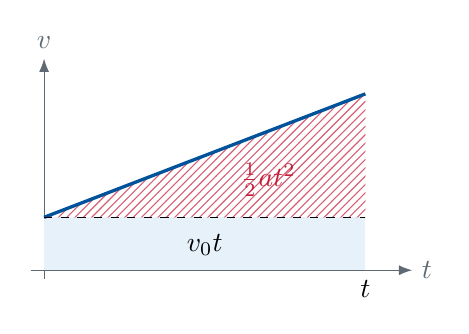
\begin{tikzpicture}[x=0.85cm,y=0.56cm,>=Latex]
      \draw[->,GraphGray] (-0.2,0)--(5.5,0) node[right]{$t$};
      \draw[->,GraphGray] (0,-0.2)--(0,4.8) node[above]{$v$};
      \fill[SoftBlue] (0,0) rectangle (4.8,1.2);
      \fill[pattern=north east lines,pattern color=ChinaRed!70]
        (0,1.2)--(4.8,4.0)--(4.8,1.2)--cycle;
      \draw[very thick,JapanBlue] (0,1.2)--(4.8,4.0);
      \draw[dashed] (0,1.2)--(4.8,1.2);
      \node at (2.4,0.58) {$v_0t$};
      \node[ChinaRed] at (3.35,2.05) {$\frac12at^2$};
      \node[below] at (4.8,0) {$t$};
    \end{tikzpicture}
    \end{center}
    \begin{alertblock}{图像含义}
      $v-t$ 图像与时间轴之间的key{有向面积}等于位移。
    \end{alertblock}
  \end{columns}
\end{frame}

% 8
\begin{frame}{第3公式：時間を消去する}
  \begin{columns}[T,onlytextwidth]
    \column{0.53\textwidth}
    \begin{block}{消去 $t$}
      \[
        \Delta x=\frac{v_0+v}{2}t,
        \qquad
        t=\frac{v-v_0}{a}
      \]
      因此
      \begin{align*}
        \Delta x
        &=\frac{v_0+v}{2}\frac{v-v_0}{a}\\
        2a\Delta x&=v^2-v_0^2
      \end{align*}
      \[
        \boxed{v^2-v_0^2=2a\Delta x}
      \]
    \end{block}
    \column{0.43\textwidth}
    \begin{alertblock}{什么时候最好用？}
      题目不给时间，或不要求时间时优先考虑。
    \end{alertblock}
    \begin{exampleblock}{制動距離}
      刹车至停止时 $v=0$：
      \[
        \Delta x=-\frac{v_0^2}{2a}
      \]
      在相同减速度下，停车距离与初速度平方成正比。
    \end{exampleblock}
  \end{columns}
\end{frame}

% 9
\begin{frame}{三つの基本公式と選び方}
  \begin{center}
  \renewcommand{\arraystretch}{1.35}
  \begin{tabular}{>{\bfseries}lccccc}
    \toprule
    公式 & $v_0$ & $v$ & $a$ & $t$ & $\Delta x$\\
    \midrule
    $v=v_0+at$ & \checkmark & \checkmark & \checkmark & \checkmark & --\\
    $\Delta x=v_0t+\frac12at^2$ & \checkmark & -- & \checkmark & \checkmark & \checkmark\\
    $v^2-v_0^2=2a\Delta x$ & \checkmark & \checkmark & \checkmark & -- & \checkmark\\
    \bottomrule
  \end{tabular}
  \end{center}
  \begin{alertblock}{选公式的步骤}
    \begin{enumerate}
      \item 先定正方向并给每个已知量加符号。
      \item 写出已知量与所求量。
      \item 选择\key{不含未知多余量}的公式。
      \item 检查单位、符号和答案的物理意义。
    \end{enumerate}
  \end{alertblock}
\end{frame}

% 10-11
\begin{frame}<1-2>{例題1：自動車の加速}
  \only<1>{
    \begin{block}{Q}
      汽车以 $5.0\unit{m/s}$ 的速度沿直线行驶，从某时刻开始以
      $2.0\unit{m/s^2}$ 的恒定加速度加速，持续 $4.0\unit{s}$。
    \end{block}
    \begin{enumerate}
      \item 求末速度。
      \item 求这段时间内的位移。
      \item 若加速度保持不变，速度达到 $17\unit{m/s}$ 时共移动了多少？
    \end{enumerate}
    \vfill
    \begin{alertblock}{先做什么？}
      取运动方向为正方向，写出 $v_0=+5.0$、$a=+2.0$。
    \end{alertblock}
  }
  \only<2>{
    \begin{block}{Q}
      $v_0=5.0\unit{m/s}$，$a=2.0\unit{m/s^2}$。求 $t=4.0\unit{s}$ 时的速度与位移，并求 $v=17\unit{m/s}$ 时的位移。
    \end{block}
    \begin{exampleblock}{解答}
      \begin{align*}
        v&=v_0+at=5.0+2.0\times4.0=13\unit{m/s},\\
        \Delta x&=v_0t+\frac12at^2
        =5.0\times4.0+\frac12\times2.0\times4.0^2
        =36\unit{m},\\
        \Delta x&=\frac{v^2-v_0^2}{2a}
        =\frac{17^2-5^2}{4}=66\unit{m}.
      \end{align*}
    \end{exampleblock}
    \begin{alertblock}{要点}
      第3问没有时间，直接使用不含 $t$ 的公式最简洁。
    \end{alertblock}
  }
\end{frame}

\section{運動のグラフ}

% 12
\begin{frame}{$x-t$ グラフ：傾きが速度}
  \begin{columns}[T,onlytextwidth]
    \column{0.56\textwidth}
    \begin{center}
    \begin{tikzpicture}[x=0.82cm,y=0.58cm,>=Latex]
      \draw[->,GraphGray] (-0.25,0)--(6.3,0) node[right]{$t$};
      \draw[->,GraphGray] (0,-0.3)--(0,5.0) node[above]{$x$};
      \draw[very thick,JapanBlue,domain=0.2:5.7,samples=50]
        plot (\x,{0.12*(\x-0.2)*(\x-0.2)+0.45});
      \coordinate (P) at (3.2,1.53);
      \fill[ChinaRed] (P) circle (2.6pt) node[above left]{$P$};
      \draw[very thick,ChinaRed] ($(P)+(-1.3,-0.78)$)--($(P)+(1.4,0.84)$)
        node[right]{接線};
      \node[JapanBlue] at (4.5,4.35) {斜率逐渐变大};
    \end{tikzpicture}
    \end{center}
    \column{0.40\textwidth}
    \begin{block}{读图}
      \[
        v=\frac{\dd x}{\dd t}
      \]
      \begin{itemize}
        \item 正斜率：$v>0$
        \item 负斜率：$v<0$
        \item 水平切线：$v=0$
        \item 曲线越来越陡：$|v|$ 增大
      \end{itemize}
    \end{block}
    \begin{alertblock}{注意}
      曲线在上方只表示 $x>0$，不代表 $v>0$。
    \end{alertblock}
  \end{columns}
\end{frame}

% 13
\begin{frame}{$v-t$ グラフ：傾きと面積}
  \begin{columns}[T,onlytextwidth]
    \column{0.57\textwidth}
    \begin{center}
    \begin{tikzpicture}[x=0.85cm,y=0.55cm,>=Latex]
      \draw[->,GraphGray] (-0.2,0)--(6.0,0) node[right]{$t$};
      \draw[->,GraphGray] (0,-1.8)--(0,4.7) node[above]{$v$};
      \fill[SoftBlue] (0,0)--(4.6,0)--(4.6,3.7)--(0,1.0)--cycle;
      \fill[SoftRed] (4.6,0)--(5.5,0)--(5.5,-0.55)--cycle;
      \draw[very thick,JapanBlue] (0,1.0)--(5.5,-0.55);
      \draw[dashed] (4.6,0)--(4.6,3.7);
      \node at (2.4,1.1) {正面积};
      \node[ChinaRed] at (5.2,-0.85) {负面积};
      \node[JapanBlue] at (2.0,3.55) {傾き $=a$};
      \fill[ChinaRed] (4.6,0) circle (2.3pt) node[below left]{转向};
    \end{tikzpicture}
    \end{center}
    \column{0.39\textwidth}
    \begin{block}{两种信息}
      \[
        a=\frac{\Delta v}{\Delta t}
      \]
      \[
        \Delta x=\int v\,\dd t
      \]
      
      斜率给加速度；与时间轴之间的有向面积给位移。
    \end{block}
    \begin{alertblock}{$v=0$}
      穿过时间轴通常表示速度方向改变。
    \end{alertblock}
  \end{columns}
\end{frame}

% 14
\begin{frame}{$a-t$ グラフ：面積が速度変化}
  \begin{columns}[T,onlytextwidth]
    \column{0.55\textwidth}
    \begin{center}
    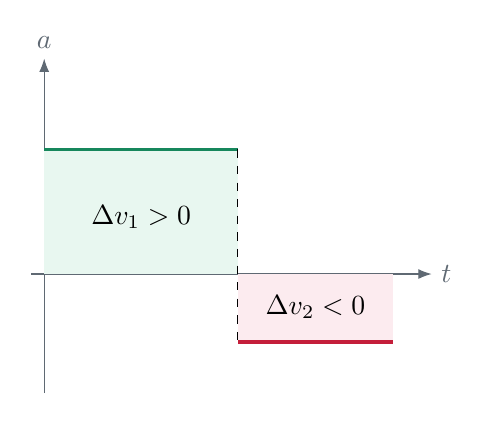
\begin{tikzpicture}[x=0.82cm,y=0.72cm,>=Latex]
      \draw[->,GraphGray] (-0.2,0)--(6.0,0) node[right]{$t$};
      \draw[->,GraphGray] (0,-2.1)--(0,3.8) node[above]{$a$};
      \fill[SoftGreen] (0,0) rectangle (3.0,2.2);
      \fill[SoftRed] (3.0,0) rectangle (5.4,-1.2);
      \draw[very thick,AccelGreen] (0,2.2)--(3.0,2.2);
      \draw[very thick,ChinaRed] (3.0,-1.2)--(5.4,-1.2);
      \draw[dashed] (3,2.2)--(3,-1.2);
      \node at (1.5,1.0) {$\Delta v_1>0$};
      \node at (4.2,-0.58) {$\Delta v_2<0$};
    \end{tikzpicture}
    \end{center}
    \column{0.41\textwidth}
    \begin{block}{面积}
      \[
        \Delta v=\int a\,\dd t
      \]
      $a-t$ 图像的有向面积等于速度变化量，而不是位移。
    \end{block}
    \begin{alertblock}{匀变速时}
      $a-t$ 图像是一条水平线；高度可正、可负，也可以为零。
    \end{alertblock}
  \end{columns}
\end{frame}

% 15
\begin{frame}{三つのグラフを対応させる}
  \small
  \begin{center}
  \renewcommand{\arraystretch}{1.35}
  \begin{tabular}{>{\bfseries}lccc}
    \toprule
    運動 & $x-t$ & $v-t$ & $a-t$\\
    \midrule
    $a=0,\ v>0$ & 上升直线 & 正的水平线 & 时间轴\\
    $a>0,\ v>0$ & 向上弯曲 & 上升直线 & 正的水平线\\
    $a<0,\ v>0$ & 向下弯曲 & 下降直线 & 负的水平线\\
    $v$ 由正变负 & 极大点 & 穿过时间轴 & 取决于斜率\\
    \bottomrule
  \end{tabular}
  \end{center}
  \begin{alertblock}{判断曲率}
    \begin{itemize}
      \item $a>0$：$x-t$ 图像开口向上
      \item $a<0$：$x-t$ 图像开口向下
      \item 转向点在 $x-t$ 图像上表现为水平切线，不一定是 $x=0$
    \end{itemize}
  \end{alertblock}
\end{frame}

% 16-17
\begin{frame}<1-2>{例題2：$v-t$ グラフの読解}
  \only<1>{
    \begin{columns}[T,onlytextwidth]
      \column{0.52\textwidth}
      \begin{center}
      \begin{tikzpicture}[x=0.75cm,y=0.55cm,>=Latex]
        \draw[->,GraphGray] (-0.2,0)--(7.0,0) node[right]{$t/\mathrm{s}$};
        \draw[->,GraphGray] (0,-3.1)--(0,4.6) node[above]{$v/(\mathrm{m/s})$};
        \draw[very thick,JapanBlue] (0,3.0)--(4,3.0)--(6,-2.0);
        \foreach \x/\lab in {4/4,6/6}{\draw (\x,0.12)--(\x,-0.12) node[below]{\lab};}
        \draw (0.12,3)--(-0.12,3) node[left]{$6$};
        \draw (0.12,-2)--(-0.12,-2) node[left]{$-4$};
      \end{tikzpicture}
      \end{center}
      \column{0.44\textwidth}
      \begin{block}{Q}
        图像表示物体的速度随时间变化。
        \begin{enumerate}
          \item $0$ 到 $4\unit{s}$ 的加速度是多少？
          \item $4$ 到 $6\unit{s}$ 的加速度是多少？
          \item 何时改变运动方向？
          \item $0$ 到 $6\unit{s}$ 的位移是多少？
        \end{enumerate}
      \end{block}
    \end{columns}
  }
  \only<2>{
    \begin{columns}[T,onlytextwidth]
      \column{0.45\textwidth}
      \begin{center}
      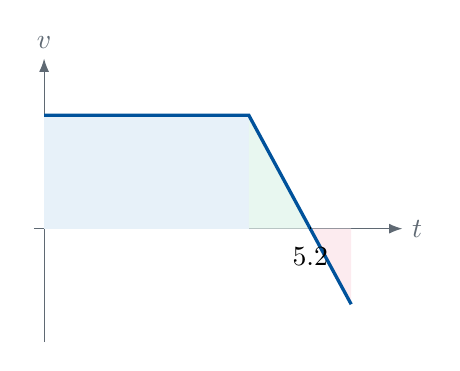
\begin{tikzpicture}[x=0.65cm,y=0.48cm,>=Latex]
        \draw[->,GraphGray] (-0.2,0)--(7.0,0) node[right]{$t$};
        \draw[->,GraphGray] (0,-3.0)--(0,4.5) node[above]{$v$};
        \fill[SoftBlue] (0,0)--(4,0)--(4,3)--(0,3)--cycle;
        \fill[SoftGreen] (4,0)--(5.2,0)--(4,3)--cycle;
        \fill[SoftRed] (5.2,0)--(6,0)--(6,-2)--cycle;
        \draw[very thick,JapanBlue] (0,3)--(4,3)--(6,-2);
        \draw[dashed] (5.2,0)--(5.2,0.05) node[below=4pt]{$5.2$};
      \end{tikzpicture}
      \end{center}
      \column{0.51\textwidth}
      \begin{exampleblock}{解答}
        \begin{enumerate}
          \item $a_1=0$。
          \item $a_2=(-4-6)/(6-4)=-5\unit{m/s^2}$。
          \item $v=0$：$6-5(t-4)=0$，故 $t=5.2\unit{s}$。
          \item 位移等于有向面积：
          \[
            \Delta x=6\times4+\frac{6+(-4)}{2}\times2
            =26\unit{m}.
          \]
        \end{enumerate}
      \end{exampleblock}
    \end{columns}
  }
\end{frame}

\section{重力による鉛直運動}

% 18
\begin{frame}{重力加速度と符号}
  \begin{columns}[T,onlytextwidth]
    \column{0.52\textwidth}
    \begin{block}{重力加速度}
      地表附近忽略空气阻力时，所有物体的加速度均竖直向下：
      \[
        g\approx9.8\unit{m/s^2}
      \]
      EJU 基础计算常给出或使用 $g=9.8$、$10\unit{m/s^2}$。
    \end{block}
    \begin{alertblock}{推荐约定}
      统一取\key{竖直向上为正方向}：
      \[
        a=-g
      \]
      自由落体、上抛、下抛都能直接使用同一套公式。
    \end{alertblock}
    \column{0.44\textwidth}
    \begin{center}
    \begin{tikzpicture}[x=1cm,y=0.85cm,>=Latex]
      \draw[->,thick,GraphGray] (0,-3.5)--(0,3.7) node[above]{$y$};
      \draw[->,ultra thick,JapanBlue] (0.7,0)--(0.7,2.8) node[right]{正方向};
      \draw[->,ultra thick,ChinaRed] (-0.7,1.8)--(-0.7,-2.5)
        node[left]{$\vec g$};
      \fill[black] (0,1.8) circle (4pt);
      \node[draw,rounded corners,fill=SoftRed] at (2.4,-1.6)
      {$a=-g$};
    \end{tikzpicture}
    \end{center}
  \end{columns}
\end{frame}

% 19
\begin{frame}{自由落下（Free Fall）}
  \begin{columns}[T,onlytextwidth]
    \column{0.52\textwidth}
    \begin{block}{定義}
      物体从静止开始，只受重力作用竖直下落：
      \[
        v_0=0,\qquad a=-g
      \]
      若以释放点为 $y_0=0$、向上为正：
      \[
        \boxed{v=-gt},\qquad
        \boxed{y=-\frac12gt^2},\qquad
        \boxed{v^2=-2gy}
      \]
    \end{block}
    \column{0.44\textwidth}
    \begin{center}
    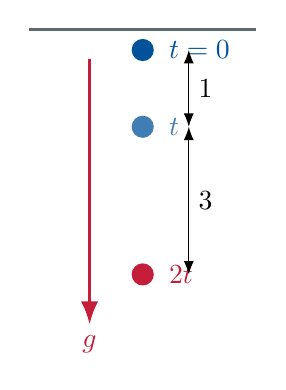
\begin{tikzpicture}[x=0.9cm,y=0.75cm,>=Latex]
      \draw[very thick,GraphGray] (-1.6,3.5)--(1.6,3.5);
      \fill[JapanBlue] (0,3.15) circle (4pt) node[right=6pt]{$t=0$};
      \fill[JapanBlue!75] (0,1.85) circle (4pt) node[right=6pt]{$t$};
      \fill[ChinaRed] (0,-0.65) circle (4pt) node[right=6pt]{$2t$};
      \draw[->,ChinaRed,very thick] (-0.75,3.0)--(-0.75,-1.5) node[below]{$g$};
      \draw[<->] (0.65,3.15)--(0.65,1.85) node[midway,right]{$1$};
      \draw[<->] (0.65,1.85)--(0.65,-0.65) node[midway,right]{$3$};
    \end{tikzpicture}
    \end{center}
    \begin{alertblock}{初始静止时}
      相邻相等时间内的位移之比为 $1:3:5:\cdots$。
    \end{alertblock}
  \end{columns}
\end{frame}

% 20-21
\begin{frame}<1-2>{例題3：自由落下}
  \only<1>{
    \begin{block}{Q}
      从高楼屋顶静止释放一个小球，忽略空气阻力，取
      $g=10\unit{m/s^2}$。小球经过 $3.0\unit{s}$ 落地。
    \end{block}
    \begin{enumerate}
      \item 求落地前瞬间速度的大小和方向。
      \item 求楼高。
      \item 求最后 $1.0\unit{s}$ 内小球下落的距离。
    \end{enumerate}
    \vfill
    \begin{alertblock}{提示}
      最后一秒位移 $=0$ 到 $3\unit{s}$ 的位移 $-$ 0 到 $2\unit{s}$ 的位移。
    \end{alertblock}
  }
  \only<2>{
    \begin{block}{Q}
      小球自由落下 $3.0\unit{s}$，$g=10\unit{m/s^2}$。求落地速度、楼高和最后一秒位移。
    \end{block}
    \begin{exampleblock}{解答}
      取向上为正：
      \begin{align*}
        v&=-gt=-30\unit{m/s},\\
        y(3)&=-\frac12\times10\times3^2=-45\unit{m},\\
        s_{\text{last}}&=\left|y(3)-y(2)\right|
        =\left|-45-(-20)\right|=25\unit{m}.
      \end{align*}
    \end{exampleblock}
    \begin{alertblock}{答案}
      速度大小 $30\unit{m/s}$，方向向下；楼高 $45\unit{m}$；最后一秒下落 $25\unit{m}$。
    \end{alertblock}
  }
\end{frame}

% 22
\begin{frame}{鉛直下方投射}
  \begin{columns}[T,onlytextwidth]
    \column{0.54\textwidth}
    \begin{block}{向上为正}
      初速度竖直向下，因此 $v_0<0$：
      \[
        v=v_0-gt
      \]
      \[
        y=v_0t-\frac12gt^2
      \]
      \[
        v^2-v_0^2=-2gy
      \]
      与自由落体的区别只有：\key{初速度不为零}。
    \end{block}
    \column{0.42\textwidth}
    \begin{center}
    \begin{tikzpicture}[x=1cm,y=0.75cm,>=Latex]
      \draw[very thick,GraphGray] (-1.5,3.2)--(1.5,3.2);
      \fill[JapanBlue] (0,2.8) circle (4pt);
      \draw[->,ultra thick,JapanBlue] (0,2.55)--(0,1.3) node[right]{$\vec v_0$};
      \draw[->,ultra thick,ChinaRed] (-0.75,2.55)--(-0.75,0.25) node[left]{$\vec g$};
      \draw[dashed,GraphGray] (0,1.1)--(0,-1.3);
      \fill[ChinaRed] (0,-1.3) circle (4pt);
      \node[draw,rounded corners,fill=SoftBlue,align=center] at (2.4,0.45)
      {速度始终向下\\且越来越大};
    \end{tikzpicture}
    \end{center}
  \end{columns}
\end{frame}

% 23-24
\begin{frame}<1-2>{例題4：鉛直下方投射}
  \small
  \only<1>{
    \begin{block}{Q}
      从距地面 $60\unit{m}$ 的位置，以 $10\unit{m/s}$ 的初速度竖直向下抛出小球。
      忽略空气阻力，取 $g=10\unit{m/s^2}$。
    \end{block}
    \begin{enumerate}
      \item 求小球落地所需时间。
      \item 求落地速度的大小。
      \item 与从同一点静止释放相比，哪一个先落地？
    \end{enumerate}
  }
  \only<2>{
    \begin{block}{Q}
      高度 $60\unit{m}$，初速度向下 $10\unit{m/s}$，$g=10\unit{m/s^2}$。
    \end{block}
    \begin{exampleblock}{解答}
      取向下为正可使计算更直接：
      \begin{align*}
        60&=10t+5t^2\\
        t^2+2t-12&=0\\
        t&=\sqrt{13}-1\approx2.61\unit{s},\\
        v&=10+10t=10\sqrt{13}\approx36.1\unit{m/s}.
      \end{align*}
    \end{exampleblock}
    \begin{alertblock}{比较}
      静止释放需要 $\sqrt{2h/g}=\sqrt{12}\approx3.46\unit{s}$，所以下抛更早落地。
    \end{alertblock}
  }
\end{frame}

% 25
\begin{frame}{鉛直上方投射：運動の三段階}
  \begin{columns}[T,onlytextwidth]
    \column{0.57\textwidth}
    \begin{center}
    \begin{tikzpicture}[x=0.9cm,y=0.75cm,>=Latex]
      \draw[very thick,GraphGray] (-2.0,-1.7)--(2.0,-1.7);
      \draw[->,thick,GraphGray] (0,-1.7)--(0,4.6) node[above]{$y$};
      \draw[->,ultra thick,JapanBlue] (-0.55,-1.25)--(-0.55,3.0)
        node[midway,left]{$v>0$};
      \draw[->,ultra thick,ChinaRed] (0.55,3.6)--(0.55,-0.9)
        node[midway,right]{$v<0$};
      \fill[JapanBlue] (0,-1.25) circle (4pt) node[right=7pt]{投射};
      \fill[black] (0,3.65) circle (4pt) node[right=7pt]{最高点 $v=0$};
      \fill[ChinaRed] (0,-1.25) circle (2pt);
      \draw[->,ChinaRed,very thick] (1.6,2.9)--(1.6,0.5) node[right]{$a=-g$};
    \end{tikzpicture}
    \end{center}
    \column{0.39\textwidth}
    \begin{block}{上升阶段}
      $v>0,\ a<0$：减速。
    \end{block}
    \begin{alertblock}{最高点}
      $v=0$，但 $a=-g\neq0$。
    \end{alertblock}
    \begin{block}{下降阶段}
      $v<0,\ a<0$：速率增大。
    \end{block}
  \end{columns}
\end{frame}

% 26
\begin{frame}{鉛直上方投射の公式}
  \begin{columns}[T,onlytextwidth]
    \column{0.51\textwidth}
    \begin{block}{基本式}
      从 $y_0=0$ 以 $v_0>0$ 向上投射：
      \[
        v=v_0-gt
      \]
      \[
        y=v_0t-\frac12gt^2
      \]
      \[
        v^2-v_0^2=-2gy
      \]
    \end{block}
    \column{0.45\textwidth}
    \begin{exampleblock}{最高点结论}
      令 $v=0$：
      \[
        t_{\mathrm{up}}=\frac{v_0}{g}
      \]
      \[
        H=\frac{v_0^2}{2g}
      \]
    \end{exampleblock}
    \begin{alertblock}{回到同一高度}
      \[
        T=\frac{2v_0}{g}
      \]
      返回时速度为 $-v_0$。
    \end{alertblock}
  \end{columns}
\end{frame}

% 27-28
\begin{frame}<1-2>{例題5：鉛直上方投射}
  \only<1>{
    \begin{block}{Q}
      从地面以 $30\unit{m/s}$ 的初速度竖直向上抛出小球，忽略空气阻力，
      取 $g=10\unit{m/s^2}$。
    \end{block}
    \begin{enumerate}
      \item 小球何时到达最高点？最高点多高？
      \item 何时回到地面？
      \item 在 $t=2\unit{s}$ 与 $t=4\unit{s}$ 时，位置和速度分别是多少？
      \item 这两个时刻有什么对称关系？
    \end{enumerate}
  }
  \only<2>{
    \begin{exampleblock}{解答}
      \begin{align*}
        t_{\mathrm{up}}&=\frac{30}{10}=3\unit{s},
        &H&=\frac{30^2}{2\times10}=45\unit{m},\\
        T&=\frac{2\times30}{10}=6\unit{s}.&&
      \end{align*}
      \[
        y(2)=30\times2-5\times2^2=40\unit{m},\quad v(2)=+10\unit{m/s},
      \]
      \[
        y(4)=30\times4-5\times4^2=40\unit{m},\quad v(4)=-10\unit{m/s}.
      \]
    \end{exampleblock}
    \begin{alertblock}{对称性}
      最高点前后等时间处位置相同，速度大小相同、方向相反。
    \end{alertblock}
  }
\end{frame}

% 29
\begin{frame}{鉛直上方投射の三つのグラフ}
  \begin{columns}[T,onlytextwidth]
    \column{0.32\textwidth}
    \centering
    \textbf{$y-t$}
    \begin{tikzpicture}[x=0.5cm,y=0.42cm,>=Latex]
      \draw[->,GraphGray] (0,0)--(5.7,0) node[right]{$t$};
      \draw[->,GraphGray] (0,-0.2)--(0,5.0) node[above]{$y$};
      \draw[very thick,JapanBlue,domain=0:5.2,samples=40]
        plot (\x,{1.75*\x-0.34*\x*\x});
      \fill[ChinaRed] (2.57,2.25) circle (2.3pt) node[above]{最高点};
    \end{tikzpicture}
    \column{0.32\textwidth}
    \centering
    \textbf{$v-t$}
    \begin{tikzpicture}[x=0.5cm,y=0.42cm,>=Latex]
      \draw[->,GraphGray] (0,0)--(5.7,0) node[right]{$t$};
      \draw[->,GraphGray] (0,-2.8)--(0,3.5) node[above]{$v$};
      \draw[very thick,ChinaRed] (0,2.5)--(5.2,-2.5);
      \fill[black] (2.6,0) circle (2.3pt) node[below]{最高点};
      \node at (3.9,2.1) {斜率 $-g$};
    \end{tikzpicture}
    \column{0.32\textwidth}
    \centering
    \textbf{$a-t$}
    \begin{tikzpicture}[x=0.5cm,y=0.42cm,>=Latex]
      \draw[->,GraphGray] (0,0)--(5.7,0) node[right]{$t$};
      \draw[->,GraphGray] (0,-2.8)--(0,3.5) node[above]{$a$};
      \draw[very thick,AccelGreen] (0,-1.8)--(5.2,-1.8) node[right]{$-g$};
    \end{tikzpicture}
  \end{columns}
  \begin{alertblock}{最高点也受重力}
    最高点只有速度瞬间为零；加速度始终为 $-g$，所以 $a-t$ 图像不会在最高点跳到零。
  \end{alertblock}
\end{frame}

\section{発展公式と結論}

% 30
\begin{frame}{平均速度と中間時刻の速度}
  \begin{columns}[T,onlytextwidth]
    \column{0.52\textwidth}
    \begin{block}{等加速度运动}
      \[
        \boxed{\bar v=\frac{v_0+v}{2}}
      \]
      又因为 $v(t)$ 随时间线性变化：
      \[
        \boxed{\bar v=v\!\left(\frac{t_1+t_2}{2}\right)}
      \]
      即某段时间的平均速度等于中间时刻的瞬时速度。
    \end{block}
    \column{0.44\textwidth}
    \begin{center}
    \begin{tikzpicture}[x=0.75cm,y=0.55cm,>=Latex]
      \draw[->,GraphGray] (0,0)--(5.7,0) node[right]{$t$};
      \draw[->,GraphGray] (0,-0.2)--(0,4.8) node[above]{$v$};
      \draw[very thick,JapanBlue] (0,1.0)--(5.0,4.0);
      \draw[dashed] (2.5,0)--(2.5,2.5);
      \draw[dashed] (0,2.5)--(2.5,2.5);
      \node[below] at (2.5,0) {$t/2$};
      \node[left] at (0,2.5) {$\bar v$};
    \end{tikzpicture}
    \end{center}
  \end{columns}
\end{frame}

% 31
\begin{frame}{等時間隔の変位差}
  \begin{columns}[T,onlytextwidth]
    \column{0.54\textwidth}
    \begin{block}{连续相等时间 $T$}
      第 $n$ 个时间段内位移：
      \[
        s_n=v_0T+\frac12a(2n-1)T^2
      \]
      相邻两段位移差为常数：
      \[
        \boxed{s_{n+1}-s_n=aT^2}
      \]
    \end{block}
    \begin{alertblock}{用途}
      纸带、频闪照片或逐秒位移题中，可直接由相邻位移差求加速度。
    \end{alertblock}
    \column{0.42\textwidth}
    \begin{center}
    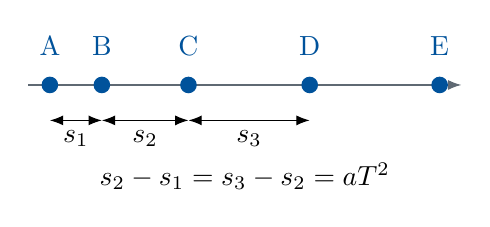
\begin{tikzpicture}[x=0.55cm,y=0.75cm,>=Latex]
      \draw[->,GraphGray] (-0.5,0)--(9.5,0);
      \foreach \x/\lab in {0/A,1.2/B,3.2/C,6.0/D,9.0/E}{
        \fill[JapanBlue] (\x,0) circle (3pt) node[above=7pt]{\lab};}
      \draw[<->] (0,-0.6)--(1.2,-0.6) node[midway,below]{$s_1$};
      \draw[<->] (1.2,-0.6)--(3.2,-0.6) node[midway,below]{$s_2$};
      \draw[<->] (3.2,-0.6)--(6.0,-0.6) node[midway,below]{$s_3$};
      \node at (4.5,-1.55) {$s_2-s_1=s_3-s_2=aT^2$};
    \end{tikzpicture}
    \end{center}
  \end{columns}
\end{frame}

% 32
\begin{frame}{第 $n$ 秒内の変位}
  \small
  \begin{block}{总位移相减}
    前 $n$ 秒总位移：
    \[
      S_n=v_0n+\frac12an^2
    \]
    第 $n$ 秒内位移：
    \begin{align*}
      s_n&=S_n-S_{n-1}\\
      &=v_0+\frac12a(2n-1)
    \end{align*}
    \[
      \boxed{s_n=v_0+\frac{a}{2}(2n-1)}
    \]
  \end{block}
  \begin{alertblock}{单位提醒}
    这个写法默认每段时间是 $1\unit{s}$。若时间间隔为 $T$，必须使用
    $s_n=v_0T+\frac12a(2n-1)T^2$。
  \end{alertblock}
\end{frame}

% 33
\begin{frame}{初速ゼロ：$1:3:5:7$ の法則}
  \begin{columns}[T,onlytextwidth]
    \column{0.51\textwidth}
    \begin{block}{$v_0=0$、每段 $1\unit{s}$}
      \[
        s_n=\frac12a(2n-1)
      \]
      因此逐秒位移之比：
      \[
        \boxed{s_1:s_2:s_3:s_4=1:3:5:7}
      \]
      前 $n$ 秒总位移：
      \[
        S_n\propto n^2.
      \]
    \end{block}
    \column{0.45\textwidth}
    \begin{center}
    \begin{tikzpicture}[x=0.7cm,y=0.55cm,>=Latex]
      \draw[->,GraphGray] (0,0)--(6.2,0) node[right]{时间段};
      \foreach \x/\h/\lab in {0.3/0.65/1,1.7/1.95/3,3.1/3.25/5,4.5/4.55/7}{
        \fill[JapanBlue!65] (\x,0) rectangle +(0.9,\h);
        \node at (\x+0.45,\h+0.35) {\lab};}
      \node at (3.0,-0.75) {每秒位移};
    \end{tikzpicture}
    \end{center}
    \begin{alertblock}{条件}
      只有初速度为零且时间间隔相等时，才能直接使用奇数比。
    \end{alertblock}
  \end{columns}
\end{frame}

% 34
\begin{frame}{制動距離と反応距離}
  \begin{columns}[T,onlytextwidth]
    \column{0.54\textwidth}
    \begin{block}{停止距离的两部分}
      \[
        d_{\text{stop}}
        =d_{\text{reaction}}+d_{\text{braking}}
      \]
      \[
        d_{\text{reaction}}=v_0t_r
      \]
      若制动减速度大小为 $A$：
      \[
        d_{\text{braking}}=\frac{v_0^2}{2A}
      \]
    \end{block}
    \column{0.42\textwidth}
    \begin{alertblock}{速度加倍}
      \begin{itemize}
        \item 反应距离变为 $2$ 倍
        \item 制动距离变为 $4$ 倍
        \item 总停车距离不会简单变为 $2$ 倍
      \end{itemize}
    \end{alertblock}
    \begin{exampleblock}{图像理解}
      反应阶段 $v$ 不变；制动阶段 $v-t$ 图像线性降到零。两段面积之和就是停车距离。
    \end{exampleblock}
  \end{columns}
\end{frame}

% 35-36
\begin{frame}<1-2>{例題6：紙テープから加速度を求める}
  \only<1>{
    \begin{block}{Q}
      打点计时器每隔 $0.10\unit{s}$ 打一个点。某物体做匀变速直线运动，连续三个相等时间段内的位移分别为
      \[
        2.0\unit{cm},\qquad3.5\unit{cm},\qquad5.0\unit{cm}.
      \]
    \end{block}
    \begin{enumerate}
      \item 判断这些数据是否符合匀变速直线运动。
      \item 求加速度。
      \item 若下一段仍保持同样运动，预测下一段位移。
    \end{enumerate}
  }
  \only<2>{
    \begin{exampleblock}{解答}
      相邻位移差：
      \[
        3.5-2.0=1.5\unit{cm},\qquad
        5.0-3.5=1.5\unit{cm}.
      \]
      差为常数，符合匀变速运动。
      \[
        a=\frac{s_{n+1}-s_n}{T^2}
        =\frac{0.015}{(0.10)^2}=1.5\unit{m/s^2}.
      \]
      下一段：
      \[
        5.0+1.5=6.5\unit{cm}.
      \]
    \end{exampleblock}
    \begin{alertblock}{单位陷阱}
      求加速度前必须把厘米换成米。
    \end{alertblock}
  }
\end{frame}

\section{総合練習}

% 37
\begin{frame}{総合練習 I：公式とグラフ}
  \small
  \begin{enumerate}
    \item 物体以 $12\unit{m/s}$ 向右运动，加速度为 $-3\unit{m/s^2}$。求停止时间和停止前位移。
    \item 某物体的 $v-t$ 图像从 $(0,8)$ 线性变化到 $(6,-4)$。求加速度、转向时刻与 $0$ 到 $6\unit{s}$ 的位移。
    \item 一辆汽车的反应时间为 $0.75\unit{s}$，初速度为 $20\unit{m/s}$，制动减速度大小为 $5.0\unit{m/s^2}$。求总停车距离。
    \item 连续 $0.20\unit{s}$ 内的位移为 $4.0\unit{cm}$、$6.4\unit{cm}$。求加速度。
  \end{enumerate}
  \begin{alertblock}{作答要求}
    写清正方向、已知量、公式和单位。
  \end{alertblock}
\end{frame}

% 38
\begin{frame}{総合練習 II：鉛直運動}
  \small
  \begin{enumerate}
    \item 小球从 $80\unit{m}$ 高处自由落下，取 $g=10\unit{m/s^2}$。求落地时间和速度。
    \item 从 $45\unit{m}$ 高处以 $10\unit{m/s}$ 竖直向下抛球。求落地速度。
    \item 从地面以 $40\unit{m/s}$ 竖直上抛小球。求最高点高度、总飞行时间及 $t=6\unit{s}$ 时的速度。
    \item 上抛球经过某高度时速度为 $+15\unit{m/s}$。再次经过同一高度时速度是多少？说明理由。
  \end{enumerate}
  \begin{alertblock}{统一处理}
    推荐取向上为正，统一写 $a=-g$；如果改取向下为正，必须从头到尾保持一致。
  \end{alertblock}
\end{frame}

% 39
\begin{frame}{総合練習：解答}
  \scriptsize
  \begin{columns}[T,onlytextwidth]
    \column{0.49\textwidth}
    \begin{block}{I}
      \begin{enumerate}
        \item $t=4\unit{s}$，$\Delta x=24\unit{m}$。
        \item $a=-2\unit{m/s^2}$，$t=4\unit{s}$ 转向，位移 $12\unit{m}$。
        \item 反应距离 $15\unit{m}$，制动距离 $40\unit{m}$，总计 $55\unit{m}$。
        \item $a=(0.064-0.040)/0.20^2=0.60\unit{m/s^2}$。
      \end{enumerate}
    \end{block}
    \column{0.49\textwidth}
    \begin{alertblock}{II}
      \begin{enumerate}
        \item $t=4\unit{s}$，速度大小 $40\unit{m/s}$，向下。
        \item $v^2=10^2+2\times10\times45$，故 $v=10\sqrt{10}\unit{m/s}$，向下。
        \item $H=80\unit{m}$，$T=8\unit{s}$，$v(6)=-20\unit{m/s}$。
        \item $-15\unit{m/s}$。同一高度处速度大小相同，下降时方向相反。
      \end{enumerate}
    \end{alertblock}
  \end{columns}
\end{frame}

% 40
\begin{frame}{重要語彙}
  \scriptsize
  \begin{columns}[T,onlytextwidth]
    \column{0.48\textwidth}
    \begin{block}{基本運動}
      \begin{tabular}{ll}
        加速度 & かそくど\\
        等加速度直線運動 & とうかそくどちょくせんうんどう\\
        初速度 & しょそくど\\
        変位 & へんい\\
        瞬間速度 & しゅんかんそくど\\
        平均速度 & へいきんそくど\\
        傾き & かたむき\\
        面積 & めんせき\\
      \end{tabular}
    \end{block}
    \column{0.48\textwidth}
    \begin{alertblock}{鉛直運動}
      \begin{tabular}{ll}
        重力加速度 & じゅうりょくかそくど\\
        自由落下 & じゆうらっか\\
        鉛直上方投射 & えんちょくじょうほうとうしゃ\\
        鉛直下方投射 & えんちょくかほうとうしゃ\\
        最高点 & さいこうてん\\
        落下時間 & らっかじかん\\
        制動距離 & せいどうきょり\\
        反応時間 & はんのうじかん\\
      \end{tabular}
    \end{alertblock}
  \end{columns}
\end{frame}

% 41
\begin{frame}{公式まとめ}
  \begin{columns}[T,onlytextwidth]
    \column{0.48\textwidth}
    \begin{block}{等加速度直線運動}
      \[
        v=v_0+at
      \]
      \[
        \Delta x=v_0t+\frac12at^2
      \]
      \[
        v^2-v_0^2=2a\Delta x
      \]
      \[
        \bar v=\frac{v_0+v}{2}
      \]
    \end{block}
    \column{0.48\textwidth}
    \begin{alertblock}{鉛直運動：上向きを正}
      \[
        a=-g
      \]
      \[
        v=v_0-gt
      \]
      \[
        y=y_0+v_0t-\frac12gt^2
      \]
      \[
        v^2-v_0^2=-2g(y-y_0)
      \]
    \end{alertblock}
  \end{columns}
  \vfill
  \centering
  \key{公式を選ぶ前に、必ず正方向と符号を決める。}
\end{frame}

% 42
\begin{frame}{参考資料}
  \small
  \begin{columns}[T,onlytextwidth]
    \column{0.49\textwidth}
    \begin{block}{EJU・高等学校物理}
      日本学生支援機構（JASSO）
      \par 日本留学試験 理科・物理 出題範囲
      \vspace{0.5em}

      文部科学省
      \par 高等学校学習指導要領「物理基礎・物理」
    \end{block}
    \column{0.47\textwidth}
    \begin{alertblock}{基礎力学}
      OpenStax
      \par \emph{University Physics, Volume 1}
      \par Chapter 3: Motion Along a Straight Line
      \vspace{0.5em}

      Halliday, Resnick and Walker
      \par \emph{Fundamentals of Physics}
    \end{alertblock}
  \end{columns}
  \vfill
  \centering
  {
    \footnotesize 日语概念用于应试，中文解释用于理解，英文术语用于补充。
  }
\end{frame}

\end{document}
